\documentclass[12pt,a4paper,utf8]{ctexart}
\usepackage{graphicx}

\usepackage{amsmath}

\usepackage{amssymb}

\usepackage{subfig}

\usepackage{cite}
\usepackage[ntheorem]{empheq}
\usepackage{enumitem}
\usepackage{fullpage}
\usepackage{cleveref}
\usepackage{cellspace}
\usepackage{listings}
\usepackage{color}
\usepackage[top=2cm, bottom=2cm, left=2cm, right=2cm]{geometry}  
\usepackage{algorithm}  
\usepackage{algorithmicx}  
\usepackage{algpseudocode}  
\renewcommand{\algorithmicrequire}{\textbf{Input:}}  % Use Input in the format of Algorithm  
\renewcommand{\algorithmicensure}{\textbf{Output:}} % Use Output in the format of Algorithm 
\definecolor{gray}{rgb}{0.5,0.5,0.5}
\definecolor{dkgreen}{rgb}{.068,.578,.068}
\definecolor{dkpurple}{rgb}{.320,.064,.680}

% set Matlab styles
\lstset{
   language=Matlab,
   keywords={break,case,catch,continue,else,elseif,end,for,function,
      global,if,otherwise,persistent,return,switch,try,while},
   basicstyle=\small\ttfamily,
   keywordstyle=\color{blue}\bfseries,
   commentstyle=\color{dkgreen},
   stringstyle=\color{dkpurple},
   backgroundcolor=\color{white},
   tabsize=4,
   showspaces=false,
   showstringspaces=false
}

\begin{document}
\CJKfamily{zhkai}	


\begin{center}
\textbf{作业三}\\
\textbf{姓名:晏瑞然~~~~~~~~~~~~~ 学号:PB19000196~~~~~~~~~~~~~~ 日期:6.8}\\
\end{center}

\begin{center}
\fbox{
\begin{minipage}{40em}
\vspace{5cm}
\hspace{20cm}
\end{minipage}}
\end{center}
\vspace{1cm}

\begin{enumerate}
\item[第一题] \textbf{本题考虑使用Richardson外推技术提高向前差商求给定函数导数的精度。}  

(a):

MATLAB程序如下:
\begin{lstlisting}[frame=single]
    % 初始化h
    h=[];
    for i =-15:0
        h=[h,10^i];
    end
    f_1=cos(1.2);% 真实值
    f_1_pred=(sin(1.2+h)-sin(1.2))./h; % 向前差商值
    err=abs(f_1-f_1_pred); % 计算误差
    % 画图
    figure
    loglog(h,err)
    \end{lstlisting}

得到结果图片如下:
\begin{figure}[H]
    \centering
    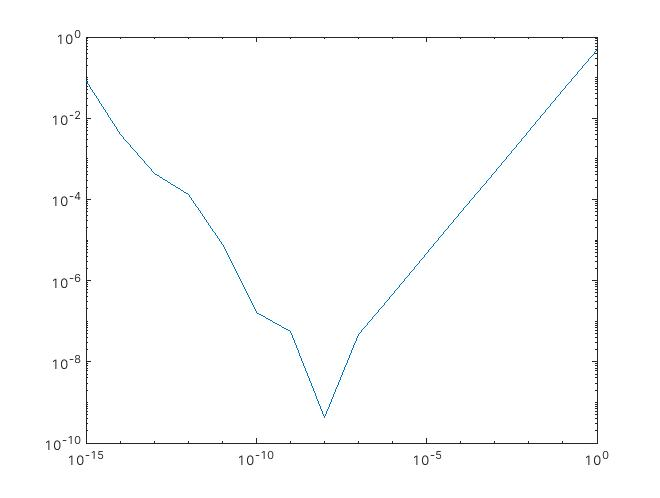
\includegraphics[width=15cm,height=8cm]{ex1a.jpg}
    \caption{第一题(a) 误差随h变化}
 \end{figure}


(b):

公式推导:

向前差分有:

$$
f(x_0+h)=f(x_0)+hf'(x_0)+\frac{h^2}{2!} f''(x_0)+\frac{h^3}{3!} f'''(x_0)+O(h^4)
$$

\begin{equation}
    R_1(h)=\frac{f(x_0+h)-f(x_0)}{h} 
    \end{equation}

由泰勒展开:
\begin{equation}
    f(x_0+h)=f(x_0)+hf'(x_0)+\frac{h^2}{2!} f''(x_0)+\frac{h^3}{3!} f'''(x_0)+O(h^4)
    \end{equation}

令:
$$
a=\frac{f''(x_0)}{2!} ,b=\frac{f'''(x_0)}{3!}  
$$
则有:
\begin{equation}
     R_1(h)=f'(x_0)+ah+bh^2+O(h^3)
\end{equation}

\begin{equation}
    R_1(\frac{h}{2} )=f'(x_0)+\frac{ah}{2} +\frac{bh^2}{4} +O(h^3)
\end{equation}

$ 2*(4)-(3) $ 得:
$$
2R_1(\frac{h}{2} )-N_1(h)=f'(x_0)-\frac{bh^2}{2} +O(h^3)
$$
$$
f'(x_0)=2R_1(\frac{h}{2} )-R_1(h)+\frac{bh^2}{2} +O(h^3)
$$
即得到一步外推公式:
$$
R_2(h)=2R_1(\frac{h}{2} )-R_1(h)
$$

第二步外推如下:
有:
\begin{equation}
    R_2(h)=f'(x_0)+a_2h^2+b_2h^3+O(h^4)
\end{equation}

\begin{equation}
    R_2(\frac{h}{2} )=f'(x_0)+\frac{a_2h^2}{4} +\frac{b_2h^3}{8} +O(h^4)
\end{equation}

其中$ a_2,b_2 $ 为常数.

由$ (4*(6)-(5))/3 $ ,与上同理得:
$$
R_3(h)=\frac{4R_2(\frac{h}{2})-R_2(h)}{3} 
$$
继续外推下去,得到:
$$
R_j=\frac{2^{j-1}R_{j-1}(\frac{h}{2} )-R_{j-1}(h)}{2^{j-1}-1} 
$$
而每次外推误差项阶数+1,故有:
$$
f'(x_0)=R_j(h)+O(h^j)
$$

算法可使用递归和非递归算法,伪代码如下:


递归算法:


\begin{algorithm}[H] 
    \caption{Richardson外推技术提高向前差商求给定函数导数的精度递归算法}  
    \label{alg1}
    \begin{algorithmic}[1] 
      \Require
       $ f $ : 待求导数值的函数;
       $ x_0 $ : 给定的求导数值的点;
       $ j $ : 外推阶数,初始值为1阶;  
       $ h $ : 向前差商的步长;  
       $ N $ : 最大外推阶数;
     \Ensure  
       $ N_j(h) $ 
       \Function{Richardson}{$ f,x_0,j,h $ }  
      \If {$j==1$} 
        \State \Return{$ \frac{f(x_0+h)-f(x_0)}{h} $};  
      \Else
        \State \Return{$ \frac{2^{j-1}Richardson(f,x_0,j-1,h/2)-Richardson(f,x_0,j-1,h)}{2^{j-1}-1} $};  
      \EndIf
      \EndFunction  
    \end{algorithmic}  
  \end{algorithm}  


  非递归算法:

\begin{algorithm}[H]
    ​\caption{Richardson外推技术提高向前差商求给定函数导数的精度非递归算法}    
    \label{alg2}​
    \begin{algorithmic}[1]  
      \Function{Richardson}{$ f,x_0,h,N,\epsilon $ }  
      \State //定义$ R_{kj}=R_j(\frac{h}{2^k} ) $ ;
      \State $ R_{00}=\frac{f(x_0+h)-f(x_0)}{h} $;  
      \State $ h_k=\frac{h}{2^k} ,k=0,1,2,\cdots ,N $ ;
      \For{k=1 to N}
      \State $ R_{k0}=\frac{f(x_0+h_k)-f(x_0)}{h_k} $ ;
      \For{j=2 to k}
      \State $ R_{kj}=\frac{2^{j-1}R_{k-1,j-1}-R_{k,j-1}}{2^{j-1}-1} $ ;
      \EndFor
      \If{$ | R_{kk}-R_{k-1,k-1} | < \epsilon $ }
      \State exit;
      \EndIf
      \EndFor
      \State \Return{$ R_{k-1,k-1} $ } ;
      \EndFunction  
    \end{algorithmic}  
  \end{algorithm}  


(c):

得到结果如下:
\begin{lstlisting}[frame=single]
>> ex1c

f_1_pred =

  -0.123542682147636
   0.362045580088605
   0.367504528760349
   0.362350201076630
   0.362356413710693
   0.362357755226488
   0.362357754488300
   0.362357754476673
   0.362357754476749
   0.362357754476749
   0.362357754476664
   0.362357754476852
   0.362357754477760
   0.362357754477841
   0.362357754479704
   0.362357754475570
   0.362357754475353
   0.362357754518873
   0.362357754506451
   0.362357754583332


err =

   0.485900436624310
   0.000312174388068
   0.005146774283675
   0.000007553400043
   0.000001340765980
   0.000000000749814
   0.000000000011627
   0.000000000000000
   0.000000000000075
   0.000000000000075
   0.000000000000010
   0.000000000000179
   0.000000000001087
   0.000000000001168
   0.000000000003030
   0.000000000001104
   0.000000000001320
   0.000000000042199
   0.000000000029777
   0.000000000106658
\end{lstlisting}

\begin{figure}[H]
    \centering
    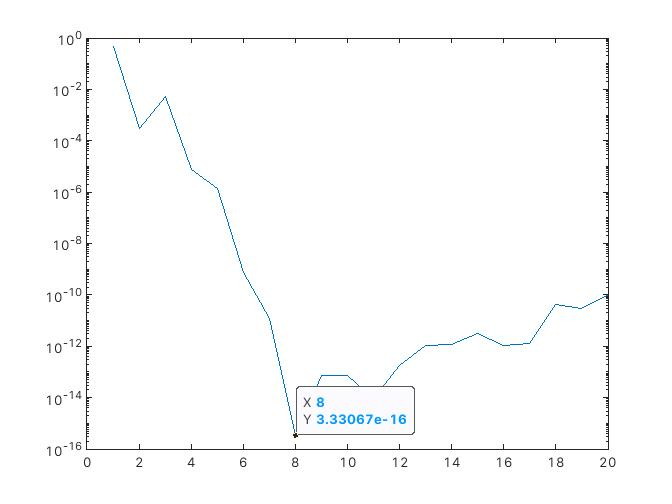
\includegraphics[width=15cm,height=8cm]{ex1c2.jpg}
    \caption{第一题(c) h=1时误差随外推次数变化}
 \end{figure}

f\_1\_pred为外推方法算出的导数值,err为误差,h的初始值为1,外推次数从1次到20次。

取最低误差的导数值作为最终值,得到外推方法算出的导数值为0.362357754476673,
误差值为$ 3*10^{-16} $ ,h初始值为1,外推次数为8(即$ R_8 $ )。

MATLAB程序如下:

主函数:(使用递归算法)
\begin{lstlisting}[frame=single]
  h=1;%设置步长
  itr=10;%迭代次数
  f_1_pred=zeros(itr,1);
  f_1=cos(1.2);%真实结果
  n=1:itr;
  %Richardson外推
  for i=1:itr
      f_1_pred(i)=Richardson(1.2,i,h);
  end
  f_1_pred %打印估算值
  err=abs(f_1_pred-f_1) %打印误差
  %画图
  figure
  semilogy(n,err)
\end{lstlisting}
函数Richardson:
\begin{lstlisting}[frame=single]
  function f=Richardson(x_0,j,h)
  if j==1 %边界
      f=(sin(x_0+h)-sin(x_0))./h;
  else %递归过程
      f=(2^(j-1)*Richardson(x_0,j-1,h/2) ...
          -Richardson(x_0,j-1,h))/(2^(j-1)-1);
  end
\end{lstlisting}





\item[第二题]\textbf{本题讨论使用复化梯形公式求周期函数的积分。}  

(a)

解:

m等分复化梯形公式为:
$$
T(h)=h[\frac{1}{2} f(a)+\sum_{i=1}^{m-1}f(a+ih)+\frac{1}{2} f(b)]
$$
当$ f(x)=cos(rx),a=-\pi ,b=\pi $ 时,带入有:


\begin{equation}
    \begin{split}
       T(h) & = h[\sum_{i=0}^{m-1}cosr(-\pi +ih)] \\
            & = h[\frac{2sin(\frac{h}{2} r)(\sum_{i=0}^{m-1}cosr(-\pi +ih))}{2sin(\frac{h}{2} r)} ] \ (sin(\frac{h}{2} r)\neq 0) \\
            & = h[\frac{-sinr((-\frac{h}{2} -\pi) ) + sinr((\frac{h}{2} -\pi +(m-1)h) )}{2sin(\frac{h}{2} r)} ]\\
            & = h[\frac{2sinr(\frac{mh}{2} )cosr(\pi -\frac{(m-1)h}{2} )}{2sin(\frac{h}{2} r)} ]\\
            & = \frac{2\pi }{m}\frac{sinr\pi \ cosr\frac{\pi}{m} }{sinr\frac{\pi}{m}} \\
            & = \frac{2\pi }{m} \frac{sinr\pi }{tanr\frac{\pi}{m} } 
          \notag
       \end{split}
\end{equation}

\begin{itemize}
\item $ r $ 不为整数时$ \lim_{m \to \infty}  \frac{2\pi }{m} \frac{sinr\pi }{tanr\frac{\pi}{m} } =\frac{2sinr\pi}{r}  $ 
与积分结果相同。

\item $ r $ 为整数时且不为m整数倍时上式为0,与结果积分相同。

\item $ r $ 为m整数倍时$ \sum_{i=0}^{m-1}cosr(-\pi +ih) $ 中 $ cosr(-\pi +ih)=cosr\pi $ 恒成立。
故最后结果为$ 2\pi cosr\pi $ 。此结果说明,若r为m的整数倍时,无法使用上述方法计算积分。
\end{itemize}

当$ f(x)=sin(rx),a=-\pi ,b=\pi $ 时,带入有:
\begin{equation}
    \begin{split}
       T(h) & = h[\sum_{i=0}^{m-1}sinr(-\pi +ih)] \\
            & = h[\frac{2sin(\frac{h}{2} r)(\sum_{i=0}^{m-1}sinr(-\pi +ih))}{2sin(\frac{h}{2} r)} ] \ (sin(\frac{h}{2} r)\neq 0) \\
            & = h[\frac{cosr((-\frac{h}{2} -\pi) ) - cosr((\frac{h}{2} -\pi +(m-1)h) )}{2cos(\frac{h}{2} r)} ]\\
            & = 0\\
          \notag
       \end{split}
\end{equation}

而原积分恒等于0,故能精确积分。

$ r $ 为整数且为m的整数倍时,$ T(h)=-mhsin(r\pi)=-2\pi sin(r\pi) $ 
此结果说明,若r为m的整数倍时,无法使用上述方法计算积分。

(b)

得到结果图片如下:

\begin{figure}[H]
  \centering
  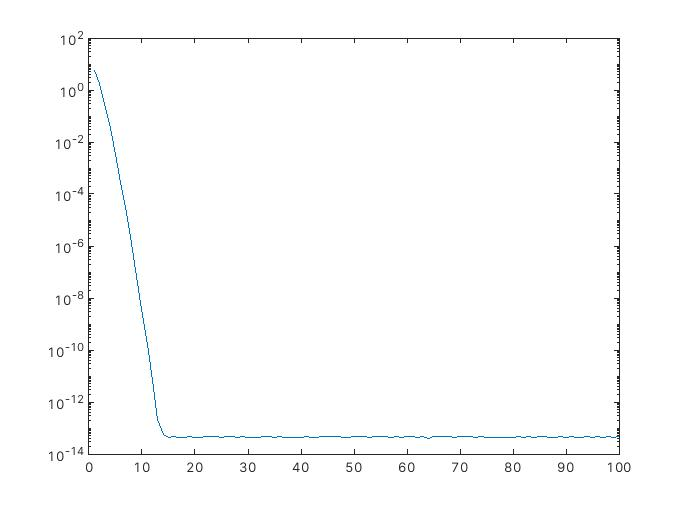
\includegraphics[width=15cm,height=8cm]{ex2b.jpg}
  \caption{第二题(b) 积分精度随着子区间数量m变化}
\end{figure}


MATLAB程序如下:
\begin{lstlisting}[frame=single]
  format long
  real_result=7.9549265210128;%真实值
  max_m=100;%设置最大区间数
  pred_result=zeros(max_m,1);%初始化
  m=1:max_m;
  for mi=1:max_m
      h=2*pi/mi;%计算步长
      %得到算法结果
      result=0.5*(exp(cos(-pi))+exp(cos(pi)));
      for i=1:mi-1
          result=result+exp(cos(-pi+i*h));
      end
      result=result*h;
      %保存结果
      pred_result(mi)=result;
  end
  %得到误差
  err=abs(pred_result-real_result);
  %画图
  figure
  semilogy(m,err)
\end{lstlisting}


\item[第三题]

(a) :

该多步法公式积分区间为$ [x_{n-1},x_{n+1}] $ ;积分节点为$ {x_{n+1},x_{n},x_{n-1}} $ .

其中,积分系数分别为:

$$
\alpha = \int_{x_{n-1}}^{x_{n+1}} \frac{(x-x_{n})(x-x_{n-1})}{(x_{n+1}-x_{n-1})(x_{n+1}-x_{n})}  \,dx =\frac{1}{3} h
$$

$$
\beta = \int_{x_{n-1}}^{x_{n+1}} \frac{(x-x_{n+1})(x-x_{n-1})}{(x_{n}-x_{n-1})(x_{n}-x_{n+1})}  \,dx =\frac{4}{3} h
$$

$$
\gamma = \int_{x_{n-1}}^{x_{n+1}} \frac{(x-x_{n+1})(x-x_{n})}{(x_{n-1}-x_{n})(x_{n-1}-x_{n+1})}  \,dx =\frac{1}{3} h
$$

得到计算格式:
$$
y_{n+1}=y_{n-1}+\frac{h}{3} [f(x_{n+1},y_{n+1}) + 4f(x_{n},y_{n}) + f(x_{n-1},y_{n-1})]
$$


(b) :

由泰勒展开可得:
$$
y(x+h)=y(x)+hy^{(1)}(x)+\frac{h^2}{2!} y^{(2)}(x)+\frac{h^3}{3!} y^{(3)}(x)+\frac{h^4}{4!} y^{(4)}(x)+\frac{h^5}{5!} y^{(5)}(x)+\cdots
$$
$$
y(x-h)=y(x)-hy^{(1)}(x)+\frac{h^2}{2!} y^{(2)}(x)-\frac{h^3}{3!} y^{(3)}(x)+\frac{h^4}{4!} y^{(4)}(x)-\frac{h^5}{5!} y^{(5)}(x)+\cdots
$$
$$
y'(x+h)=y^{(1)}(x)+hy^{(2)}(x)+\frac{h^2}{2!} y^{(3)}(x)+\frac{h^3}{3!} y^{(4)}(x)+\frac{h^4}{4!} y^{(5)}(x)+\frac{h^5}{5!} y^{(6)}(x)+\cdots
$$
$$
y'(x-h)=y^{(1)}(x)-hy^{(2)}(x)+\frac{h^2}{2!} y^{(3)}(x)-\frac{h^3}{3!} y^{(4)}(x)+\frac{h^4}{4!} y^{(5)}(x)-\frac{h^5}{5!} y^{(6)}(x)+\cdots
$$

而根据微分方程可得计算格式为
$$
y(x_n+h)=y(x_n-h)+\frac{h}{3} [y'(x_n+h)+4y'(x_n)+y'(x_n-h)]
$$

将上述泰勒展开带入,取$ x=x_n $ 得
$$
T_{n+1}=-\frac{1}{90} h^5y^{(5)}
$$

(c) :

解函数如下:
\begin{figure}[H]
  \centering
  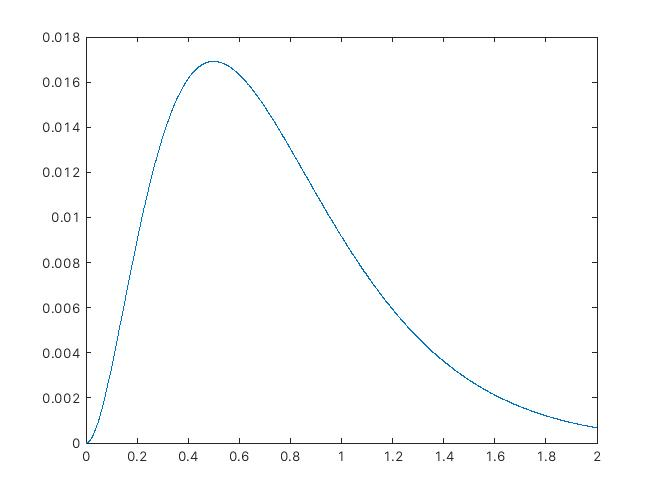
\includegraphics[width=15cm,height=8cm]{ex3c.jpg}
  \caption{第三题(c) 解函数图像}
\end{figure}

MATLAB程序如下:
\begin{lstlisting}[frame=single]
  h=0.001;% 设置步长
  x=0:h:2;
  y=zeros(1,size(x,2));
  % 得到多步法系数
  alpha=1/3*h;
  beta=4/3*h;
  gamma=1/3*h;
  y(1)=0;%初始值
  %RUNGE-KUTTA方法
  k1=x(1)*exp(-4*x(1))-4*y(1);
  k2=(x(1)+h/2)*exp(-4*(x(1)+h/2))-4*(y(1)+h/2*k1);
  y(2)=y(1)+h*k2;
  %多步转移
  for i=3:size(x,2)
      y(i)=1/(4*alpha+1)*( ...
          y(i-2)+alpha*x(i)*exp(-4*x(i)) ...
          +beta*(x(i-1)*exp(-4*x(i-1))-4*y(i-1)) ...
          +gamma*(x(i-2)*exp(-4*x(i-2))-4*y(i-2))...
          );
  end
  %画图
  figure
  plot(x,y)  
\end{lstlisting}

(d):

求精确解:
$$
y'=xe^{-4x}-4y
$$
移项可得
$$
e^{4x}y'+4ye^{4x}=x
$$
于是有
$$
(ye^{4x})'=x
$$
两边积分得
$$
y=\frac{1}{2} x^2e^{-4x}+Ce^{-4}
$$
带入初始条件$ y(0)=0 $ 得
$$
y=\frac{1}{2} x^2e^{-4x}
$$
算得精确解在2处值为:6.7093e-04

loglog图如下:
\begin{figure}[H]
  \centering
  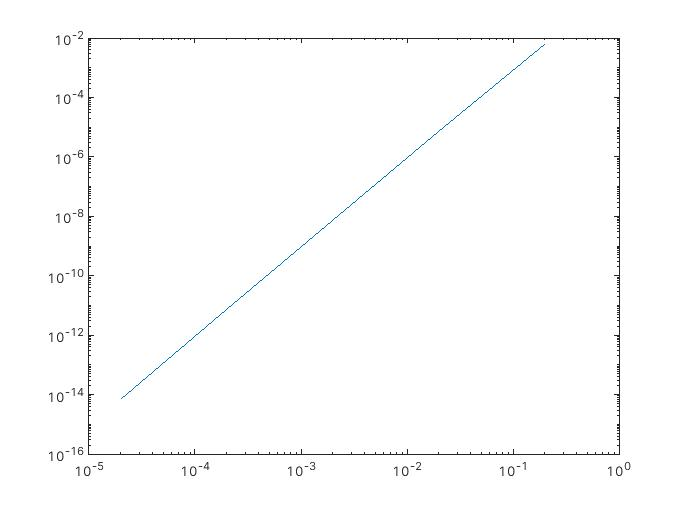
\includegraphics[width=15cm,height=8cm]{ex3d.jpg}
  \caption{第三题(d) loglog图展现阶数}
\end{figure}

下对改图进行解释:

该图横座标是步长h,纵座标是得出结果与真实结果误差。
取loglog后可以发现其是直线。
由k阶误差满足
$$
T_{k}=\alpha h^k+O(h^{k+1})\ \ \ \  \alpha =const
$$
可知,直线的斜率就是误差阶数。
图中斜率为3,故误差阶数为3,精度阶数即为2阶。
这也很好解释,因为所用Runge-Kutta方法为2阶,而精度只取决于最低阶精度,
因为最低阶的误差才是误差阶数,比最低阶误差大的误差都远小于最低阶误差。
故最终结果的精度阶数为2阶。

MATLAB程序如下:
\begin{lstlisting}[frame=single]
  pred=[];
  n=[];
  for i=1:5
      n=[n 10^i];
  end
  h=2./n;
  for j=1:size(n,2)
      hi=1/n(j);
      x=0:hi:2;
      y=zeros(1,size(x,2));
      %得到多步法系数
      alpha=1/3*hi;
      beta=4/3*hi;
      gamma=1/3*hi;
      y(1)=0;%初始值
      %RUNGE-KUTTA
      k1=x(1)*exp(-4*x(1))-4*y(1);
      k2=(x(1)+hi/2)*exp(-4*(x(1)+hi/2))-4*(y(1)+hi/2*k1);
      y(2)=y(1)+hi*k2;
      %多步转移
      for i=3:size(x,2)
          y(i)=1/(4*alpha+1)*( ...
              y(i-2)+alpha*x(i)*exp(-4*x(i)) ...
              +beta*(x(i-1)*exp(-4*x(i-1))-4*y(i-1)) ...
              +gamma*(x(i-2)*exp(-4*x(i-2))-4*y(i-2))...
              );
      end
      y(size(x,2))
      pred = [pred y(size(x,2))];%记录结果
  end
  y2_real=0.5*2^2*exp(-4*2);%得到真实值
  err_y2=abs(pred-y2_real);%计算误差
  %画图
  figure
  loglog(h,err_y2)
\end{lstlisting}


\end{enumerate}




\end{document}
